
\documentclass[border=3pt,tikz]{standalone}
\begin{document}
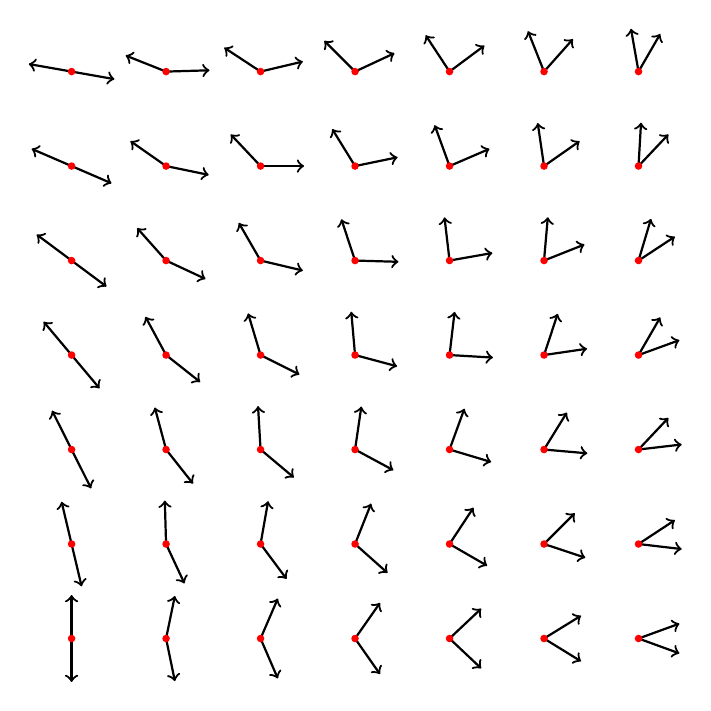
\begin{tikzpicture}[scale=1.2]
  \def\N{7}
  \foreach \i [evaluate={\y=\i-0.5}] in {1,...,\N}{
    \foreach \j [evaluate={\x=\j-0.5;
                           \ang=80*(\i-1)/(\N-1); % seperation
                           \dang=90-70*(\j-1)/(\N-1); % boost
                 }] in {1,...,\N}{
      \draw[->,thick] (\x,\y) --++ (\ang-\dang:0.46); % bottom jet
      \draw[->,thick] (\x,\y) --++ (\ang+\dang:0.46); % top jet
      \fill[red] (\x,\y) circle(0.04);
    }
  }
\end{tikzpicture}
\end{document}
